\section{Date: 2026-11-07}
\noindent \textbf{Series ID: NORRECDM} 

\noindent This series is titled OECD based Recession Indicators for Norway from the Peak through the Trough (DISCONTINUED) and has a frequency of Daily, 7-Day. The units are +1 or 0 and the seasonal adjustment is Not Seasonally Adjusted.The observation start date is 1960-02-01 and the observation end date is 2022-09-30.The popularity of this series is 2. \\ 

\noindent \textbf{Series ID: MORTMRGN5NE} 

\noindent This series is titled Margin for 5/1-Year Adjustable Rate Mortgage in the Northeast Freddie Mac Region (DISCONTINUED) and has a frequency of Weekly, Ending Thursday. The units are Percent and the seasonal adjustment is Not Seasonally Adjusted.The observation start date is 2005-01-06 and the observation end date is 2015-12-31.The popularity of this series is 1. \\ 

\subsection{Raw Regression}
\noindent Regresses the two series against each other directly. A significant result here can come just as easily from both series sharing a long-run trend as from any real relationship.

\begin{center}
\begin{tabular}{lclc}
\toprule
\textbf{Dep. Variable:}        & value\_fred\_MORTMRGN5NE & \textbf{  R-squared:         } &     0.174   \\
\textbf{Model:}                &           OLS            & \textbf{  Adj. R-squared:    } &     0.172   \\
\textbf{Method:}               &      Least Squares       & \textbf{  F-statistic:       } &     120.2   \\
\textbf{Date:}                 &     Sat, 07 Nov 2026     & \textbf{  Prob (F-statistic):} &  1.63e-25   \\
\textbf{Time:}                 &         17:03:06         & \textbf{  Log-Likelihood:    } &    1072.5   \\
\textbf{No. Observations:}     &             574          & \textbf{  AIC:               } &    -2141.   \\
\textbf{Df Residuals:}         &             572          & \textbf{  BIC:               } &    -2132.   \\
\textbf{Df Model:}             &               1          & \textbf{                     } &             \\
\textbf{Covariance Type:}      &        nonrobust         & \textbf{                     } &             \\
\bottomrule
\end{tabular}
\begin{tabular}{lcccccc}
                               & \textbf{coef} & \textbf{std err} & \textbf{t} & \textbf{P$> |$t$|$} & \textbf{[0.025} & \textbf{0.975]}  \\
\midrule
\textbf{const}                 &       2.7734  &        0.002     &  1388.819  &         0.000        &        2.769    &        2.777     \\
\textbf{value\_fred\_NORRECDM} &      -0.0351  &        0.003     &   -10.963  &         0.000        &       -0.041    &       -0.029     \\
\bottomrule
\end{tabular}
\begin{tabular}{lclc}
\textbf{Omnibus:}       & 54.533 & \textbf{  Durbin-Watson:     } &    0.276  \\
\textbf{Prob(Omnibus):} &  0.000 & \textbf{  Jarque-Bera (JB):  } &  314.645  \\
\textbf{Skew:}          &  0.052 & \textbf{  Prob(JB):          } & 4.74e-69  \\
\textbf{Kurtosis:}      &  6.626 & \textbf{  Cond. No.          } &     2.44  \\
\bottomrule
\end{tabular}
%\caption{OLS Regression Results}
\end{center}

Notes: \newline
 [1] Standard Errors assume that the covariance matrix of the errors is correctly specified.

\begin{figure}
\centering
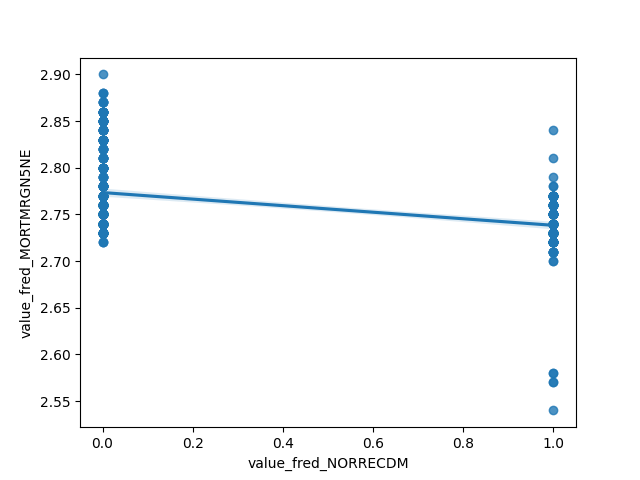
\includegraphics[scale = 0.9]{plots/plot_2026-11-07.png}
\caption{Raw Regression Plot for 2026-11-07}
\end{figure}
\newpage
\subsection{Detrended Regression}
\noindent Regresses the residuals of each series after removing its own linear time trend, so a shared trend can no longer drive the result on its own. A relationship that stays significant here is better evidence of a genuine link between the two series.

\begin{center}
\begin{tabular}{lclc}
\toprule
\textbf{Dep. Variable:}                   & value\_fred\_MORTMRGN5NE\_detrended & \textbf{  R-squared:         } &     0.220   \\
\textbf{Model:}                           &                 OLS                 & \textbf{  Adj. R-squared:    } &     0.219   \\
\textbf{Method:}                          &            Least Squares            & \textbf{  F-statistic:       } &     161.6   \\
\textbf{Date:}                            &           Sat, 07 Nov 2026          & \textbf{  Prob (F-statistic):} &  8.78e-33   \\
\textbf{Time:}                            &               17:03:06              & \textbf{  Log-Likelihood:    } &    1186.5   \\
\textbf{No. Observations:}                &                   574               & \textbf{  AIC:               } &    -2369.   \\
\textbf{Df Residuals:}                    &                   572               & \textbf{  BIC:               } &    -2360.   \\
\textbf{Df Model:}                        &                     1               & \textbf{                     } &             \\
\textbf{Covariance Type:}                 &              nonrobust              & \textbf{                     } &             \\
\bottomrule
\end{tabular}
\begin{tabular}{lcccccc}
                                          & \textbf{coef} & \textbf{std err} & \textbf{t} & \textbf{P$> |$t$|$} & \textbf{[0.025} & \textbf{0.975]}  \\
\midrule
\textbf{const}                            &    2.243e-13  &        0.001     &  1.75e-10  &         1.000        &       -0.003    &        0.003     \\
\textbf{value\_fred\_NORRECDM\_detrended} &      -0.0334  &        0.003     &   -12.712  &         0.000        &       -0.039    &       -0.028     \\
\bottomrule
\end{tabular}
\begin{tabular}{lclc}
\textbf{Omnibus:}       & 209.063 & \textbf{  Durbin-Watson:     } &    0.410  \\
\textbf{Prob(Omnibus):} &   0.000 & \textbf{  Jarque-Bera (JB):  } & 2385.406  \\
\textbf{Skew:}          &  -1.266 & \textbf{  Prob(JB):          } &     0.00  \\
\textbf{Kurtosis:}      &  12.661 & \textbf{  Cond. No.          } &     2.05  \\
\bottomrule
\end{tabular}
%\caption{OLS Regression Results}
\end{center}

Notes: \newline
 [1] Standard Errors assume that the covariance matrix of the errors is correctly specified.

\begin{figure}
\centering
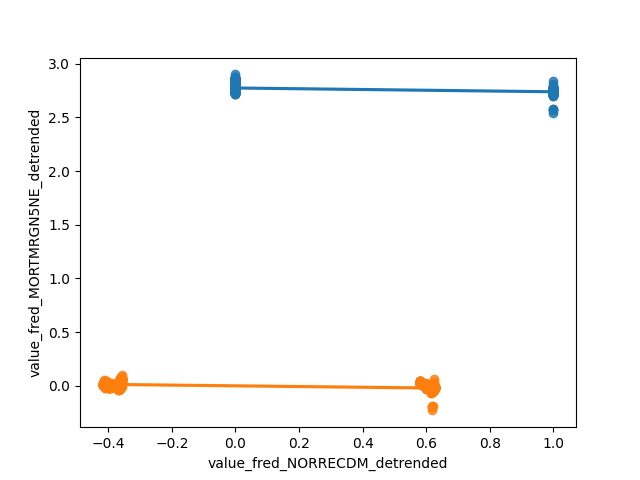
\includegraphics[scale = 0.9]{plots/plot_2026-11-07_detrended.png}
\caption{Detrended Regression Plot for 2026-11-07}
\end{figure}
\newpage
